%%%%%%%%%%%%%%%%%%%%%%%%%%%%%%%%%%%%%%%%%
% Simple Sectioned Essay Template
% LaTeX Template
%
% This template has been downloaded from:
% http://www.latextemplates.com
%
% Note:
% The \lipsum[#] commands throughout this template generate dummy text
% to fill the template out. These commands should all be removed when 
% writing essay content.
%
%%%%%%%%%%%%%%%%%%%%%%%%%%%%%%%%%%%%%%%%%

%----------------------------------------------------------------------------------------
%	PACKAGES AND OTHER DOCUMENT CONFIGURATIONS
%----------------------------------------------------------------------------------------

\documentclass[12pt]{article} % Default font size is 12pt, it can be changed here
\usepackage{geometry} % Required to change the page size to A4
\geometry{a4paper,left=2cm,right=2.0cm,top=2.5cm,bottom=2.5cm} % Set the page size to be A4 as opposed to the default US Letter
\usepackage[toc,page]{appendix}
\usepackage{graphicx} % Required for including pictures
\usepackage{booktabs}
\usepackage{float} % Allows putting an [H] in \begin{figure} to specify the exact location of the figure
\usepackage{wrapfig} % Allows in-line images such as the example fish picture
\usepackage{fancyhdr}
\usepackage{lipsum} % Used for inserting dummy 'Lorem ipsum' text into the template
\usepackage{lastpage}
\usepackage[ruled,vlined]{algorithm2e}
\usepackage{caption}
\usepackage{subfigure}
\usepackage{palatino}
\usepackage[table,xcdraw]{xcolor}
\linespread{1.1} % Line spacing
\graphicspath{{Pictures/}} % Specifies the directory where pictures are stored
\pagestyle{fancy}
\title{MCM/ICM Template}

\begin{document}
	\lhead{Team \# 1901279}
\rhead{Page \thepage \ of \pageref{LastPage}}
\cfoot{}
\maketitle
\thispagestyle{fancy}
\tableofcontents % Include a table of contents
\newpage % Begins the essay on a new page instead of on the same page as the table of contents 


\section{Introduction} % Major section
\subsection{Problem Background} % Sub-section
[Problem Background] see in problem background.tex

%----------------------------------


\subsection{Our Work} % Sub-section
[Our Work] See in OurWork.tex

\begin{equation}
E=mc^2+\sqrt{E}
\end{equation}

\section{Assumptions} % Major section
[Assumptions] see file Assumptions.tex

\section{Notations} % Major section
[Notations] see in Notations.tex

%-------------------------------
The following variables will be defined here here as they are widely used throughout this paper. Additional variables might be defined later, but restricted to a particular section.

\begin{table}[H]
	\centering
	\begin{tabular}{|c|c|}
		\hline
		\rowcolor[HTML]{656565} 
		{\color[HTML]{FFFFFF} \textbf{Symbol}} & {\color[HTML]{FFFFFF} \textbf{Definition}} \\ \hline
		i    & the $i_{th}$ item in a series of unsigned integer numbers  \\ \hline
		i    & the $i_{th}$ item in a series of unsigned integer numbers  \\ \hline
		i    & the $i_{th}$ item in a series of unsigned integer numbers  \\ \hline
		i    & the $i_{th}$ item in a series of unsigned integer numbers  \\ \hline
		i    & the $i_{th}$ item in a series of unsigned integer numbers  \\ \hline
	\end{tabular}
	\caption{Notations}
\end{table}


\section{Statement of our Model} % Sub-section
[ModelStatement] see in ModelStatement.tex


\section{Implementation}	 % Sub-sub-section
[Implementation] see in Implementation.tex

%------------------------------------------------

\section{Model Analysis} % Sub-sub-section
\subsection{Sensitivity Analysis}
\subsection{Strengths and Weaknesses}
\subsubsection{Strengths}
\subsubsection{Weaknesses}

\section{Conclusion} % Major section

\newpage
\section{Letter}

Dear Sir or Madam,
Yours Faithfully,
Team \# 1901279	



%----------------------------------------------------------------------------------------
%	BIBLIOGRAPHY
%----------------------------------------------------------------------------------------
\newpage
\begin{thebibliography}{99} % Bibliography - this is intentionally simple in this template

\bibitem{1}
Figueredo, A.~J. and Wolf, P. S.~A. (2009).
\newblock Assortative pairing and life history strategy - a cross-cultural
  study.
\newblock {\em Human Nature}, 20:317--330.
 
\end{thebibliography}

%----------------------------------------------------------------------------------------
\newpage
\appendix
\appendixpage
\section{Mathematical Backgrounds}
\newpage
\section{EXAMPLES(TO BE DELETED!)}
% use http://www.tablesgenerator.com/latex_tables
\begin{table}[H]
	\centering
	\begin{tabular}{@{}llr@{}}
		\toprule
		\toprule
		\multicolumn{2}{c}{Item} &            \\ \cmidrule(r){1-2}
		Animal     & Description & Price (\$) \\ \midrule \midrule
		Gnat       & per gram    & 13.65      \\
		& each        & 0.01       \\
		Gnu        & stuffed     & 92.50      \\
		Emu        & stuffed     & 33.33      \\
		Armadillo  & frozen      & 8.99       \\ \bottomrule
	\end{tabular}
	\caption{My caption}
	\label{my-label}
\end{table}

\begin{figure}[H] % Example image
	\center{
\includegraphics[width=0.5\linewidth]{placeholder}}
	\caption{Example image.}
	\label{fig:speciation}
\end{figure}

\lipsum[6] % Dummy text
\begin{wrapfigure}{l}{0.4\textwidth} % Inline image example
	\begin{center}
		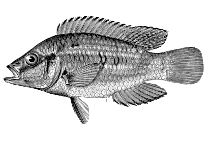
\includegraphics[width=0.38\textwidth]{fish}
	\end{center}
	\caption{Fish}
\end{wrapfigure}
\lipsum[7-8] % Dummy text

\begin{figure}[H]
	\centering
	\subfigure[Original]{
		\begin{minipage}[t]{0.25\linewidth}
			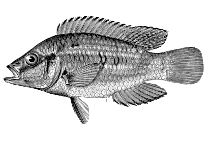
\includegraphics[width=1.4in]{fish}
		\end{minipage}
	}
	\subfigure[SIFT Features]{
		\begin{minipage}[t]{0.25\linewidth}
			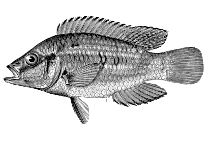
\includegraphics[width=1.4in]{fish}
		\end{minipage}
	}
	\caption{Source Image}
\end{figure}

\begin{description} % Numbered list example
	
	\item[First] \hfill \\
	\lipsum[9] % Dummy text
	
	\item[Second] \hfill \\
	\lipsum[10] % Dummy text
	
	\item[Third] \hfill \\
	\lipsum[11] % Dummy text
	
\end{description} 


%ALGORITHMS
\IncMargin{1em}
\LinesNumbered
\begin{algorithm}[H]
	\SetKwData{Left}{left}\SetKwData{This}{this}\SetKwData{Up}{up}
	\SetKwFunction{Union}{Union}\SetKwFunction{FindCompress}{FindCompress}
	\SetKwInOut{Input}{input}\SetKwInOut{Output}{output}
	
	\KwData{this text}
	\KwResult{how to write algorithm with \LaTeX2e }
	
	
	\BlankLine
	\While{not at end of this document}{
		read current\;
		\eIf{understand}{
			go to next section\;
			current section becomes this one\;
		}{
			go back to the beginning of current section\;
		}
	}
	\caption{How to write algorithms}
	
\end{algorithm}
\DecMargin{1em}
	


\end{document}